\documentclass[12pt]{article}
\newcommand{\ts}{\textsuperscript}

\usepackage[margin=1in]{geometry}
\usepackage{caption}
\usepackage{cite}
\usepackage{subcaption,graphicx}
\usepackage{lineno, blindtext}
\usepackage{float}
\usepackage{color}
\usepackage{graphicx}
\usepackage[hidelinks]{hyperref}
\usepackage{enumitem}
\usepackage{multicol}
\usepackage{fancyhdr}
\usepackage{times}
\usepackage{mathtools}
\usepackage{pdfpages}
\setlength{\parindent}{0pt}
\newcommand{\forceindent}{\leavevmode{\parindent=1em\indent}}
%\usepackage{siunitx}
\usepackage{chronology}

\title{MSE 486\\Directed Study Proposal\\ \bigskip \textbf{2 Player Texas Hold'em Poker\\Reinforcement Learning Python Bot}}
\author{Ryan Fielding - 301284210\\rafieldi@sfu.ca\\778.886.8199}
\date{April $10^{th}$, 2020}

\begin{document}

\maketitle
\newpage

{\Large \textbf{Abstract\\\\}}
This paper outlines the project proposal for a directed study in machine learning, through implementation and development of an AI based bot to learn and understand different strategies to play poker. Particularly, the game of Texas Hold'em will be the basis for this project, potentially beginning with Leduc Hold'em since it is a much simpler version of the game.\\\\
To initiate the project, the first couple weeks will be dedicated to project research, pertaining to coding language, type of machine learning to implement, project goals, requirements and more. Most likely, the development will be done in Python, with the implementation of reinforcement learning.\\\\
To elaborate on the overall development, first, a basic poker environment will be initialized. There is no need to develop this from scratch as there are plenty of sources to implement a gaming environment in many languages. Following, basic bots will need to be setup, as well as strategic bots and honest bots. Each level of bot will get more and more advanced, and then the remaining few will implement the different types of machine learning.\\\\
Training these bots will mostly consist of self play and reward based learning, however other strategies will be researched, including that of DeepStack, Libratus, Pluribus and many others that are successfully based on machine learning. The reason for two player poker, instead of 3,4 or even 6, is because with a lower number of players at play, a rule based gaming strategy is far more effective, and much easier to implement and train. As the number of players increase, the game becomes a multi-player game that requires more sophisticated strategies and potentially even player modelling.\\\\
This report discusses background, learning outcomes, the proposed project, a timeline, and other information. 

\newpage

\section{Background}
The complex game of poker requires reasoning with hidden information. When one plays a game, not only do they 'quantify' the value of their own hand, they also aim to predict what cards the opposing players hold. Other players can even bet high when they're hand is not valuable at all, a strong tactic called \textit{bluffing}. Additionally, there are other factors that weigh in, including pot size, call size, remaining stack and more. For background information on Texas Hold'em and how it is played, see the reference \cite{tex}.\\\\
\begin{figure}[H]
    \centering
    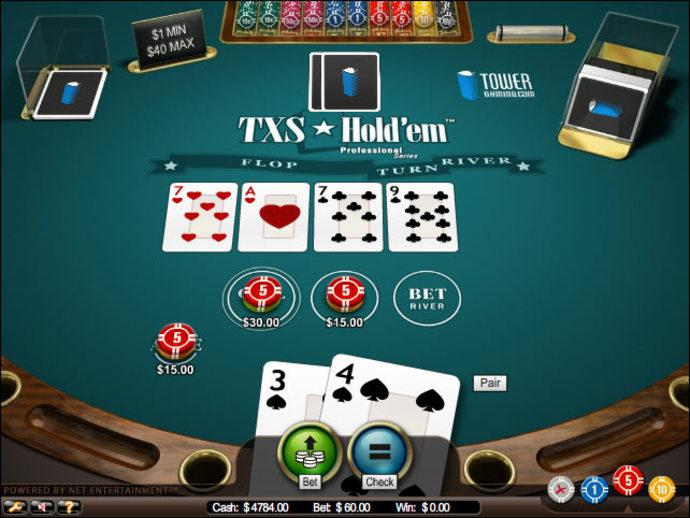
\includegraphics[width=.70\linewidth]{figures/texas.jpg}
    \caption{Online Texas Hold'em}
    \label{fig:tex}
\end{figure}
2 player Texas Hold'em presents an excellent opportunity to implement machine learning, as rule based strategies work fairly well, according to many experienced sources \cite{ai}. Game theory, with higher numbers of players, is far less helpful. Additionally, this becomes incredibly computationally expensive as it drastically increases the number of possibilities, making it much harder to make a sound decision at the time of it's turn. Bots known as Libratus and DeepMind's Go bot used 100 CPU's and 2000 CPU's, respectively \cite{ai}. However, a much less expensive AI has been developed, known as \textit{Pluribus}, which only required 2 CPU's to run. It was developed via reinforcement learning and self play, and such a tactic will most definitely be employed for the development of this project. 
\section{Learning Outcomes}
This study serves as to produce many learning outcomes, which have been listed below.
\begin{itemize}
	\item Machine learning research and understanding of the many different types, pros and cons, hardships and more.
	\item Machine learning implementation, development process and uses in practice.
	\item Coding language development in the language of choice, most likely Python.
	\item Reinforcement learning, training, action enhancement and more.
	\item Numerous strategies to play Texas Hold'em, though this is only a bi-product.
\end{itemize}

\section{Proposed Project}
Overall, the project will aim to implement reinforcement learning strategies with training through self play. There are many other machine learning techniques that can be applied to this project, however they are computationally expensive. The goal is to create a bot, that learns through playing itself, how it could have made more money through different actions, and potentially even how to 'play the man', not the game, which would require the implementation of a rapid learning function to understand it's opponent's strategy, aggressive, defensive, and more.
\subsection{Reinforcement Learning}
The motivation for this type of learning lies in it's low computational expensiveness. Imagine you are playing chess, before you make a move, you are thinking what all the other player's potential moves are, even 2 or 3 moves ahead of the present. For a computer to do this, in a game with many possibilities and many players, it is incredibly expensive to do in a short period of time. Reinforcement learning is "an area of machine learning concerned with how software agents ought to take actions in an environment in order to maximize the notion of cumulative reward" \cite{rl}.
\begin{figure}[H]
    \centering
    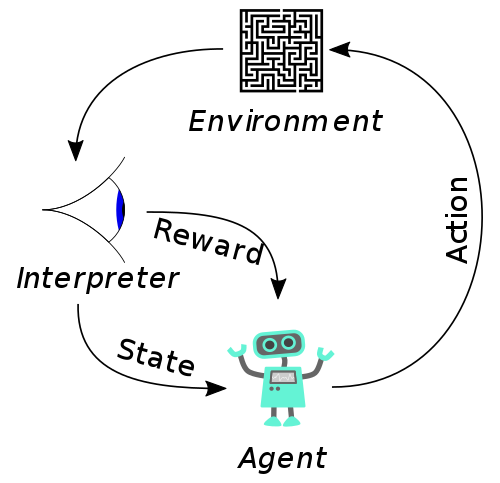
\includegraphics[width=.50\linewidth]{figures/rel.png}
    \caption{A Typical Reinforcement Learning Scenario \cite{rl}}
    \label{fig:rl}
\end{figure}
If you are familiar with the game of poker, the image shown above is nearly directly applicable to the game. Thus, implementing this type of learning, coupled with iterative self play, can lead to a very powerful poker playing bot, especially in two player poker. Potential for implementation in more than two player poker may be explored and tested depending on effectiveness of that of two player.
\section{Other Information}
\subsection{Timeline}
\begin{chronology}[3]{1}{15}{\textwidth}
\event{1}{Project Kick-off}
\event[1]{3}{Research}
\event[2]{4}{Environment Development}
\event{4}{Basic Environment and Bots Implemented}
\event{6}{Console Based UI Gameplay for Testing}
\event[4]{6}{RL Dev. and Training}
\event[5]{10}{Training and Testing}
\event{7}{Revision 1. Complete - RL}
\event{8}{More Advanced RL AI Bot}
\event[10]{14}{Testing, Training, Competitive Play}
\event{14}{Project Completion}
\event[14]{15}{Documentation}

\end{chronology}
\textbf{Project Timeline for the Summer 2020 Semester, by Week}\\

\subsection{Contact Hours}
I can be contacted via my cell phone or email from the hours of 9am-8pm, Monday to Friday. Meetings can be set at any time if it fits a schedule for both parties.
\subsection{Meeting Schedules}
Meetings will be set with the associated supervising professor for once every two weeks, to ensure consistent progress, development and results, as well as advice and insight.
\subsection{Grading Scheme}
This will be based off any faculty grading templates that are available.


% ADD BIBLIOGRAPHY
\nocite{*}
\bibliographystyle{IEEE/IEEEtran}
\bibliography{IEEE/IEEEabrv,IEEE/biblio}

\end{document}
